%% -*- coding: utf-8 -*-
\documentclass[12pt,pagesize,paper=landscape,paper=192mm:108mm]{scrbook} 
%1920x1080 1280x720
\areaset[current]{192mm}{108mm}
\usepackage{calc}
\usepackage[T2A]{fontenc}
\usepackage[utf8]{inputenc}
\usepackage[english,russian]{babel}
\usepackage{microtype}
\usepackage{misccorr}
\usepackage{cmap}
%\usepackage[unicode=true]{hyperref}
\usepackage{graphicx}
\usepackage{amssymb}
\usepackage{amsmath}
%\usepackage{srcltx}
\usepackage{textcomp}
\usepackage{xspace}
%научные символы и смайлики \smiley \frownie
\usepackage{wasysym}
\usepackage{ccicons}
\begin{document}
\begin{titlepage}
  \vspace*{-0.5em}
  \begin{center}    
    \hspace*{3em}
    \begin{minipage}[t]{3em}
      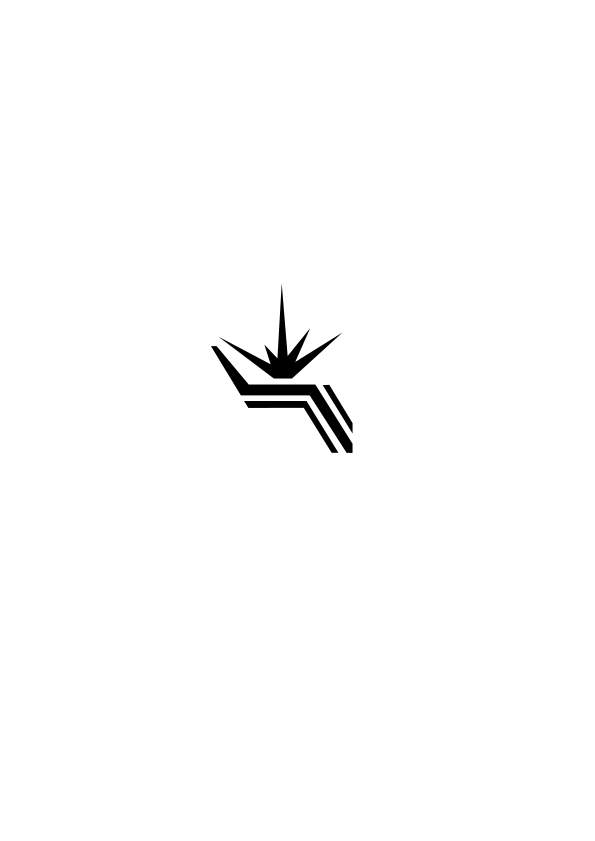
\includegraphics[width=\textwidth]{../BINP-logo}
    \end{minipage}\hfill
    \begin{minipage}{0.23\linewidth}
    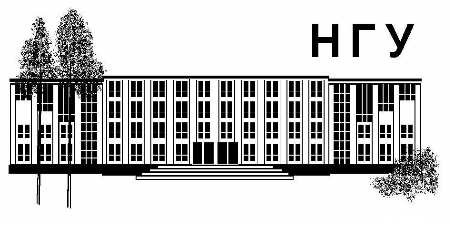
\includegraphics[width=\textwidth]{../NSU-logo}
    \end{minipage}
    \hfill
    \hspace*{6em}

    Кафедра теоретической физики физического факультета НГУ
    \medskip

    \Large
    Профессор Фадин В.\,С.
    \bigskip

    \huge
    \textbf{Квантовая электродинамика}
    \bigskip

    \Large
    Лекция № 10
    \vfill

    \normalsize
    % \begin{minipage}{0.65\linewidth}
    % \end{minipage}
    \vfill

    \normalsize \ccbysa\hspace{0.5em}  Новосибирск 2013
  \end{center}
\end{titlepage}
\vspace*{-1em}
\begin{center}
\vfill
  \begin{minipage}{0.8\linewidth}
    Проинтегрированная по углам вероятность излучения мягкого
    фотона. Расходимость при интегрировании по частоте
    фотона. Переосмысление теории возмущения, неправильность
    постановки задачи о вычислении сечений с определенными конечным
    состояний, отсутствие процессов с участием заряженных частиц без
    излучения фотонов. Инфракрасные расходимости, регуляризация
    введением массы фотона, размерностная регуляризация.  Суммирование
    радиационных поправок, связанных с виртуальными мягкими фотонами,
    во всех порядках теории возмущения. Среднее число реальных мягких
    фотонов, вероятность излучения определенного числа фотонов,
    пуассоновское распределение по числу излученных
    фотонов. Сокращение инфракрасных расходимостей. Смысл борновского
    сечения как сечения процесса с излучением любого числа
    фотонов. Физически наблюдаемое сечение. Пределы применимости
    мягкофотонного приближения в виртуальных поправках и
    экспериментальные ограничения на частоту фотона в реальных
    поправках. Особые случаи: процесс аннигиляции $e^+e^-$ с рождением
    резонансов, аккутратный учет излучения в начальном состоянии.
  \end{minipage}
  \vfill

  % \normalsize \ccbysa\hspace{0.5em} Новосибирск 2013
\end{center}
\end{document}
